\raggedright
\mychapter{2}{Work Project 2}
	\label{ch:opt}
	\section{Esercizio 1: Evolutionary Optimization}
		\label{sec:es1}
		\subsection{Esperimento 1: Ottimizzazione}
			Attraverso gli algoritmi forniti siamo stati in grado di sperimentare le differenti tecniche di \emph{ricerca locale} su diversi problemi. Esse si basano sul principio dei miglioramenti successivi: si cerca in primo luogo una soluzione,anche non ottima, ed in seguito ci si concentra sull'ottimizzazione. Va considerato che spesso si riesce a determinare solo un massimo locale, ottenendo risultati più o meno soddisfacenti a seconda dell'applicazione.
			\subsubsection{Random Searching}
				Questo algoritmo prevede semplicemente la determinazione casuale di un insieme di soluzioni e la comparazione dei relativi costi per l'identificazione di quella a costo minimo.\par
				Abbiamo effettuato differenti esperimenti variando il numero di soluzioni estratte casualmente: ad un suo eccessivo aumento non si ottengono necessariamente risultati nettamente migliori da giustificare l'evidente incremento della complessità computazionale in termini temporali; d'altro canto, un numero esiguo di soluzioni produce risultati dalla qualità incostante.
			\subsubsection{Hill Climbing}
				L'\texttt{Hill Climbing} inizialmente determina una soluzione ed i suoi "vicini", se uno di essi presenta un costo migliore della soluzione corrente,verrà scelta questa come l'attuale  alla prossima iterazione, attuando, in tal modo, il processo dei miglioramenti successivi; se la soluzione corrente ha costo minore dei suoi vicini, termina la serie di miglioramenti iterativi poiché si è in presenza di un massimo locale (minimo locale rispetto al costo, in quanto una soluzione è preferibile da un altra se il costo è minore o maggiore dipende dal problema).\par
				Vari esperimenti ci hanno condotto a risultati decisamente migliori del \texttt{Random Searching}, che sottolineano la maggior efficienza dell'\texttt{Hill Climbing}. La variabilità nella qualità della soluzione, al seguito di svariate esecuzioni, è dipendente dai massimi locali del problema specifico,infatti partendo da situazioni iniziali diversi, arriviamo a valori diversi.
			\subsubsection{Simulation annealing}
				Versione rivisitata dell' L'\texttt{Hill Climbing}, questo metodo di ottimizzazione è ispirato dal riscaldamento termico di una lega e al suo successivo raffreddamento. Viene comparata la soluzione corrente ad una determinata casualmente (nel nostro caso tramite un cambiamento di quella corrente): l'algoritmo tende a spostarsi sempre verso una soluzione successiva migliore, solo con una certa probabilità verso quelle peggiori, che tenderà a diminuire col tempo. Questa probabilità dipende dalla qualità della soluzione successiva: mosse pessime avranno minore probabilità. Viene, inoltre, introdotto un concetto di "temperatura": essa determina la probabilità di spostarsi verso soluzioni non ottime. Inizialmente questo valore sarà alto (temperatura elevata), in seguito essa tenderà a calare (raffreddamento), consentendo, in ultima battuta, la scelta della soluzione ottimizzata. Tale probabilità è data dalla seguente espressione:
				\begin{equation*}
				{\LARGE e^{\frac{-(costosuccessivo+costoattuale)}{temperatura}}}
				\end{equation*}
				Osserviamo che con l'abbassamento della temperatura, ad ogni iterazione dell' algoritmo, tale probabilità decresce.
				Le ragioni alla base di questa logica risiedono nella maggiore possibilità di trovare un massimo globale, evitando che ci si possa assestare su un punto di massimo locale come una \emph{spalla} (shoulder).\par
				Dalle prove sperimentali abbiamo constatato risultati migliori o uguali all'\texttt{Hill Climbing}, appurando la maggiore capacità di ottenere soluzioni con costo inferiore.
				
				% $e^{-(migliorcosto+costoattuale/temperatura)}$ dove, più ci avviciniamo alla soluzione(diminuzione dei costi) e Tale strategia ha senso, , invece così facendo possiamo trovare anche soluzioni migliori.
			\subsubsection{Genetic Algorithms}
				Ulteriore algoritmo che tenta di superare i limiti dell'\texttt{Hill Climbing} è quello genetico. Esso è ispirato dalla natura, proponendo un'evoluzione delle soluzioni tipicamente darwiniana. L'algoritmo prende le mosse selezionando un insieme casuale di soluzioni, detto \emph{popolazione}. Gli esemplari di questa vengono poi valutati ed ordinati attraverso una \emph{funzione di fitness} (rappresentata nel nostro caso dal costo minimo). Nell'implementazione utilizzata, si procede alla creazione della successiva \emph{generazione} a partire da un prestabilito numero di migliori soluzioni. Attraverso il processo di \emph{elitarismo} quelle ottime sopravviveranno nella nuova generazione; la restante popolazione sarà costituita attraverso la \emph{mutazione} (cambiamento casuale ad una soluzione) ed il \emph{crossover} (combinazione di due soluzioni) dell'elite.\par
				Vari esperimenti di hanno portato a riscontrare risultati simili  al \texttt{Simulated Annealing}, se non migliori in taluni casi, che presentano, però, una minore variabilità con misure ripetute. Riusciamo, in definitiva, ad ottenere una buona ottimizzazione, di qualità superiore all'\texttt{Hill Climbing} ed al \texttt{Random Searching}.
		\subsection{Esperimento 2: Caso d'uso}
			L'ottimizzazione sulla quale ci vogliamo concentrare è quella di una funzione $F(x)$, così definita:
			\[
				F(x)=
				\begin{cases}
					10 & \mbox{se }x<5.2\\
					x^2 & \mbox{se }5.2\leq x \leq 20\\
					x-1 & \mbox{se } x>20
				\end{cases}
				\mbox{ ; }x \in [-100,100]
			\]
			dove la $x$ può assumere valori tra $[-100,100]$. La ricerca di tale valore verrà effettuata tramite algoritmo genetico. Prima di tutto, però, dobbiamo definire la funzione di costo, così da poter determinare quando la nostra soluzione tende a migliorare o, viceversa, a peggiorare:
			\bigskip
			\begin{python}
		def costmax(sol):
			if sol[0]>100 or sol[0]<-100:
				cost=0
			else:
				cost=F(sol)
		return cost  
			\end{python}
			\bigskip
			La nostra funzione di costo è definita nel seguente modo: se il valore di cui si calcola il costo non è accettabile, poiché nel passaggio tra una generazione ad un'altra si è avuto un esemplare della popolazione non voluto, cioè non accettabile per la soluzione (valore al di fuori dell' intervallo $[-100,100]$ ), gli si dà un costo pari a 0, in modo tale che per la creazione della prossima generazione non verrà preso in considerazione; altrimenti il costo è dato dall'applicazione della F sul valore in ingresso.\par
			L' algoritmo prima di tutto genera una popolazione iniziale scegliendo a caso valori presi nello spazio delle soluzioni, ne calcola i vari score e sceglie una elite di individui (quelli che in questo caso massimizzano lo score), dopodiché, per un numero di generazioni volute, possiamo far mutare un elemento o fare il crossover tra due di essi in base ad una probabilità di mutazione da noi fornita. \par 
			Abbiamo però riscontrato un problema nella rappresentazione numerica: i dati vengono passati all' algoritmo sotto forma di float, che non permette di definire un' operazione di mutazione o crossover semplice. Per ovviare a questo inconveniente i numeri vengono convertiti nella loro forma binaria (in questo caso a 32 bit), definendo quindi la mutazione come il cambiamento di un bit da 1 a 0, o viceversa.\par
			Il crossover è eseguito scegliendo un numero di bit casuale da una soluzione e il numero restante di bit da un'altra, affinché si riottenga un codice di 32 bit. Possiamo vedere il crossover come un'operazione di ricombinazione genetica in cui parte del materiale genetico di un individuo si ricombina con un altro. Così facendo, ad ogni cambio generazionale, si genera una progenie come combinazione di geni dei genitori migliori della generazione precedente, attuando in tal modo una selezione naturale.\par
			La mutazione, invece, è un fattore casuale che permette di introdurre nuovi tratti negli individui, di variarne i geni, donando in tal modo alla progenie caratteristiche distintive non presenti nei genitori e consentendo alla specie di attuare un processo evolutivo che favorisca la sopravvivenza.
			%non saprei se mettere un esempio di soluzione o un grafico, ditemi voi%
			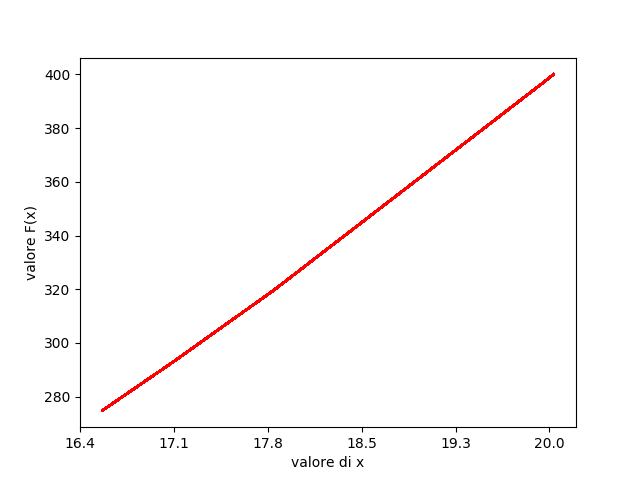
\includegraphics[scale=0.80]{fitness.png}
			Come si può vedere, il valore che ottimizza la F(x) tende a x=20. Il risultato si riesce a trovare anche partendo da una popolazione iniziale ristretta a soli 100 elementi. Per un numero di iterazioni discreto (100 in questo caso) la soluzione non solo viene trovata, ma viene confermata più volte, dimostrando che, anche se si provano nuove combinazioni, l'esemplare che massimizza la fitness è stato già trovato precedentemente e le iterazioni successive non fanno altro che confermarlo.
	\section{Esercizio 2: MDS: Visually Exploring US Senator Similarity}
		\label{sec:es2}
			\subsubsection{Clustering}
				Il Clustering, o analisi di raggruppamento, è una tecnica di intelligenza artificiale volta alla selezione e raggruppamento di elementi omogenei in un insieme di dati. Tutte le tecniche di clustering si basano sul concetto di distanza tra due elementi, che ci permette di definire il concetto di somiglianza tra gli elementi. Infatti l'appartenenza o meno ad un insieme dipende da quanto l'elemento preso in esame sia distante dall'insieme. La bontà delle analisi ottenute dagli algoritmi di clustering dipende dalla metrica: metriche diverse porteranno quasi certamente a cluster differenti.
				
			\subsubsection{MDS: MultiDimensional Scaling}
				Il MultiDimensional Scaling è una tecnica di analisi statistica usata per mostrare graficamente le differenze o somiglianze tra elementi di un insieme. È una generalizzazione del concetto di ordinamento: partendo da un matrice contenente le informazioni che vogliamo analizzare e moltiplicandola per la sua trasposta, otterremo una matrice quadrata reppresentante la "somiglianza"  di ogni elemento con un altro, dopodiché l'algoritmo di scaling multidimensionale assegnerà a ogni soggetto una posizione in uno spazio N-dimensionale, con N stabilito a priori tramite una metrica.
			\subsubsection{Riflessioni }		
				%	Nel codice che ci e' stato fornito un abbiamo a disposizione due esempi, il primo, un  si basa su il giudizio da parte di quattro clienti  riguardo a 6 prodotti,
				L'esempio affrontato descrive l'orientamento politico dei membri dei Congressi americani, dal 101-esimo al 111-esimo, sull' analisi dei voti.
				%Lo scopo è quello di raggruppare i venditori i senatori in base alle loro preferenze.
				Sono utilizzati i dataset in formato \emph{STATA}, programma commerciale di calcolo statistico diffuso tra gli accademici nell'ambito delle scienze politiche. Essi presentano i voti delle differenti sedute dei 10 Congressi presi in esame. 
				La metrica utilizzata per la distanza è quella euclidea.
				%Dal Multidimensional scaling del primo esempio giungiamo alla seguente conclusione :" i recensori A e D hanno valori di metrica abbastanza vicini tra loro mentre per i recensori B e C no.
				%Analizzando i dati che abbiamo a disposizione non rimaniamo sorpresi di questi risultati,l'algoritmo classifica A e D come simili infatti hanno espresso quattro pareri concordanti su sei, mentre B e C hanno espresso solo due concordanti e non è un buon risultato per classificarli come simili.
				%Ovviamente per considerazioni più approfondite abbiamo bisogno di un numero maggiore di dati."
				Essendo i dati troppo complessi e strutturati per i nostri scopi, per facilitare l' analisi viene eseguita una semplificazione aggregando dei tipi di voto: tra tutte le possibili classi di votazione (nove in totale) se ne ricavano solo tre.\par
				Viene dapprima analizzato il caso del 110-esimo Senato. Notiamo che gli schieramenti dei voti sono netti: Repubblicani a destra e Democratici a sinistra.
				%Successivamente abbiamo lo stesso grafico con i nomi dei senatori che appartengono ad un determinato partito ed effettuando delle ricerche su internet notiamo che l' orientamento politico discrimina la votazione , per esempio Obama si trova nel lato dei Repubblicano mentre Jeffords, il cui ha un passato da Repubblicano, comunque mantiene quellì orientamento anche se ora è un indipendente.
				Estendendo l'analisi a tutti i Congressi, constatiamo che le scelte di voto sono consistenti con il partito di appartenenza. Alcuni grafici possono sembrare meno polarizzati, caratterizzati da punti più centrali, come se i voti siano stati meno radicali, ma tale risultato si ottiene perché non si ha una scala univoca che definisca la distanza.
				% quindi gli estremismi sono presenti sempre.
				%da vedere meglio come esprimere questo risultato
	\section{Esercizio 3: Constraint Satisfaction Problems}
		\label{sec:es3}
		Il problema di soddisfacimento dei vincoli che ci ritroviamo ad affrontare è il seguente: "Un agente intelligente  deve colorare le province della regione Campania evitando che le confinanti abbiano lo stesso colore". Questo è un tipico esempio di domanda a cui si può rispondere con algoritmi che tengono conto del soddisfacimento dei vincoli. Come prima cosa formalizziamo il problema :
		\begin{lstlisting}
Variabili: Caserta, Benevento, Napoli, Avellino, Salerno
Vincoli: province confinanti devono avere colori diversi
		\end{lstlisting}
		Possiamo, dunque, ricavare il grafo dei vincoli, i cui nodi sono le variabili ed i cui archi connettono coppie di attributi che partecipano ad un vincolo. In questo caso i vincoli sono binari, cioè sono coinvolti soltanto due nodi per ogni vincolo.
		\begin{center}
			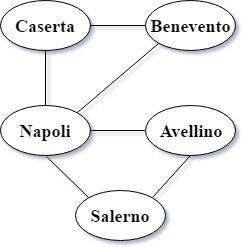
\includegraphics[scale=0.7]{ConstraintGraph.jpg}
		\end{center}
		Analizziamo il caso in cui l'agente disponga di solo 2 colori.
		\begin{lstlisting}
Dominio = {Colore1, Colore2}
		\end{lstlisting}
		Questo significa che le variabili possono assumere solo due colori.
		Da uno sguardo attento del grafo possiamo formalizzare un ulteriore vincolo, non binario: le variabili Napoli, Benevento e Avellino devono essere necessariamente tutte diverse (non sono l'unica tripla che rispetta questo vincolo).
		Un dominio formato da solo due colori non ci permetterà mai di poter soddisfare questo vincolo, pertanto il problema non è risolvibile. 
		Ma oltre questa formulazione formale abbiamo provato anche l'algoritmo di \texttt{Backtracking Search}, attraverso il quale si perviene presto alla conclusione dell'impossibilità di risolvere il problema vincolato. Ad esempio, applicando le euristiche per migliorare l'efficienza della ricerca, assegniamo a Napoli (\texttt{Degree Heuristic}: variabile con più vincoli sulle rimanenti variabili) il valore Colore1; se procediamo assegnando Colore2 a Caserta (o qualsiasi altra variabile dato che ora presentano tutte un solo valore ammissibile), si ottiene un fallimento, poiché tramite il \texttt{Forward Checking} si osserva che Benevento non può assumere nessun valore ammissibile. Questa risultato è comune anche agli altri path dell'albero di ricerca e tutto ciò è intuitivamente comprensibile poiché con soli 2 colori non siamo in grado di soddisfare i loop di 3 nodi presenti nel grafo dei vincoli.\par
		\bigskip
		Analizziamo il caso in cui l'agente disponga di 3 colori.
		\begin{lstlisting}
Dominio = {Colore1, Colore2, Colore3}
		\end{lstlisting}
		%Sorcando la cresta dell'esecuzione dell'algoritmo
		Proviamo ora l'algoritmo con il dominio di dimensione maggiore. Partiamo da Napoli assegnandole il Colore1 e notiamo che questa scelta riduce i valori ammissibili per le altre province confinanti a due. Coloriamo, ora, Benevento con il Colore2; di conseguenza Caserta sarà la nostra prossima scelta poiché le si può assegnare solo un colore, il Colore3. Tale scelta è dettata dall'euristica che abbiamo applicato, il \texttt{Minimum Remaining Values}, che prevede la scelta della variabile con numero minimo di valori possibili. Ad Avellino, non confinante con Caserta, le possiamo assegnare il Colore3 senza produrre nessun conflitto. A Salerno, infine, assegniamo il Colore2.\par 
		Osserviamo che ogni provincia ha un colore diverso dalle confinanti, ma queste ultime  possono essere colorate allo stesso modo nel caso in cui non siano a loro volta adiacenti. Possiamo, in conclusione, affermare che è possibile soddisfare i vincoli dato questo dominio.
		\begin{center}
			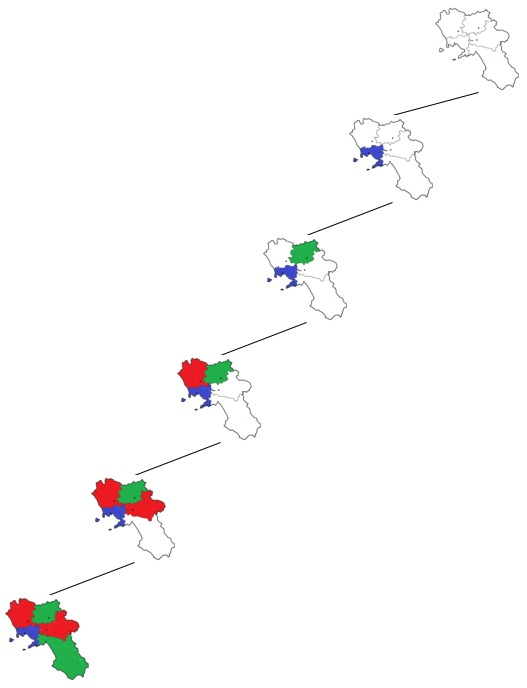
\includegraphics[width=0.6\textwidth, height=0.4\textheight]{SearchTree.jpg}
		\end{center}\par
		Anche il caso con quattro colori sicuramente permetterà di soddisfare i vincoli perché si è aumentato il numero di valori ammissibili lasciando invariate le informazioni iniziali. Verifichiamo che sia così.
		\begin{lstlisting}
Dominio = {Colore1, Colore2, Colore3, Colore4}
		\end{lstlisting}
		La prima provincia che coloriamo è Napoli, assegnandole il Colore1: così facendo riduciamo tutti i colori possibili per le altre province, avendo Napoli il maggior numero di vincoli. Avellino sarà la nostra prossima scelta: assegnandole il Colore2 diminuirà anche il numero di valori per Salerno e Benevento. Passiamo a Caserta: essa può assumere tutti i valori tranne Colore1. Osserviamo, però, che l'assegnazione dei valori Colore3 e Colore4 produrrebbe una diminuzione del dominio degli attributi che possiamo assegnare a Benevento. Applichiamo il \texttt{Least Constraining Value}, euristica che predilige il valore che lascia più libertà alle variabili adiacenti, e scegliamo il Colore2 per  Caserta. Segue Benevento con il Colore3 e Salerno con il Colore3. Si noti che, per le ultime due scelte, si può effettuare una scelta completamente arbitraria tra Colore3 e Colore4.\par
		Come ci si poteva aspettare, l'aggiunta di un nuovo elemento nel Dominio, senza l'alterazione dei vincoli, permette ugualmente la risoluzione del problema, perfino evitando di utilizzare il nuovo valore. Possiamo, allora, dedurre che, una volta trovata la soluzione con un determinato numero di valori, essa esisterà anche per un Dominio più esteso.\par 
		In quest'ultimo caso, però, si può parlare di vincoli più "elastici", più rilassati, grazie ai maggiori gradi di libertà per la determinazione della soluzione. Ad esempio, con un Dominio di tre elementi il numero di soluzioni possibili sicuramente sarà molto più limitato rispetto ad uno con quattro elementi, che permette più opportunità di scelta. Possiamo, quindi, affermare che le soluzioni relative al Dominio esteso includano quelle del compatto. 
	\section{Esercizio 4}
		\label{sec:es4}
		Ricerchiamo un possibile approccio per trovare la soluzione con l' ausilio di algoritmi genetici al problema vincolato con $card(Dominio)=4$. Prima di utilizzare gli algoritmi genetici per risolvere il problema, dobbiamo definire una funzione di costo. Tra le tanti possibili scelte, abbiamo optato per la seguente: 
		\begin{equation*}
			\mbox{costo }=\mbox{ numero di conflitti}
		\end{equation*}
		dove il conflitto è inteso come due province confinanti con lo stesso colore. Una soluzione sarà quindi valutata rispetto ad una funzione di fitness che prende in considerazione il numero di conflitti: quanto più una soluzione presenterà un costo minore, tanto più assumerà un valore di fitness maggiore. Ovviamente ottimizzare la soluzione significa minimizzare il valore assunto dalla funzione di costo. Poiché essa può assumere solo valori positivi, la migliore soluzione riscontrabile avrà costo nullo.\par
		Particolarizziamo l'algoritmo genetico per il problema in esame. La popolazione iniziale sarà costituita da un insieme di mappe che presentano una colorazione casuale delle province. Definiamo, poi, una probabilità di mutazione che consente di variare casualmente colore ad una provicia, tra i tre rimanenti (escludendo il colore attualmente assegnato). Tale operazione permette di aggiungere caratteristiche che la nostra popolazione iniziale non aveva, ottenendo maggiore varietà nel processo di generazione affinché si testino anche soluzioni non necessariamente eccellenti. Ora non ci resta che definire l'operazione di crossover, che consiste nel prendere in modo casuale dall'elite due elementi (mappe colorate) e scegliere probabilisticamente il numero di province di uno, da unire con le restanti dell'altro. %Serve un finale più ad effetto, una conclusione. Io non credo che l'algoritmo arrivi sempre ad una soluzione del problema vincolato: cioè cerca di ottimizzare la soluzione con meno conflitti, ma se poi essa ne presenta anche uno solo non vale come soluzione al problema vincolato: riusciamo solo ad ottimizzare la soluzione al problema rilassato e, se siamo fortunati, può capitare che essa sia soluzione anche per quello vincolato (il cui spazio delle soluzioni è contenuto in quello del problema rilassato).
		%CONSULTAZIONE per un'aggiunta: bisogna mutare solo i colori delle province che generano conflitti o li prendiamo a caso? Lo stesso vale per il crossover: prendiamo solo le parti buone? Il problema da una parte è che in questo modo stiamo "veicolando" il processo di selezione naturale, lo stiamo forzando come se mettessimo i pokemon nella pensione per ottenere le uova. Dall'altra parte, però, cerchiamo di apparare i conflitti, anche se c'è sempre l'eventualità che introduciamo, mutando o ricombinando, nuovi conflitti con le parti che prima erano buone.
		%-----------------------------------------------
		%Un approccio possibile per trovare la soluzione con l' ausilio di algoritmi genetici potrebbe essere questo:
		%Definire come funzione di costo il numero di conflitti, province confinanti con lo stesso colore generano un conflitto. Il nostro obiettivo è quindi quello di minimizzare questo valore.\par 
		%La popolazione iniziale sarà costituita da un insieme di cartine colorate in modo casuale. Definiamo una probabilità di mutazione,se non siamo in quest' ultimo caso allora avverrà l' operazione di crossover che consiste nel prendere in modo casuale dall' elite due elementi e scegliere probabilisticamente, quanti cromosomi(province) di uno, da unire con i restanti dell' altro,nel caso  della mutazione invece basterà scegliere un elemento dalla cartina e cambiarli colore a scelta tra gli altri tre, escludendo ovviamente quello già assegnato.
		